\documentclass{beamer}
\mode<presentation>
\usepackage{amsmath, amssymb, mathtools}
\usepackage{graphicx}
\usepackage{enumitem}
\usepackage{multicol}
\usepackage{adjustbox}
\usepackage{url}
\usepackage{listings}
\usepackage{gvv}
\def\UrlBreaks{\do\/\do-}
\usetheme{Boadilla}
\usecolortheme{lily}
\setbeamertemplate{footline}
{
  \leavevmode%
  \hbox{%
  \begin{beamercolorbox}[wd=\paperwidth,ht=2.25ex,dp=1ex,right]{author in head/foot}%
    \insertframenumber{} / \inserttotalframenumber\hspace*{2ex} 
  \end{beamercolorbox}}%
  \vskip0pt%
}
\setbeamertemplate{navigation symbols}{}

\title{Probability}
\author{Dwarak A - EE24BTECH11019}
\date{\today} 

\begin{document}

\begin{frame}
    \titlepage
\end{frame}

\section*{Outline}
\begin{frame}
    \tableofcontents
\end{frame}

\section{Problem Statement}
\begin{frame}
    \frametitle{Problem Statement}
    Given:
    \begin{align}
        P(A) &= 0.25 \\
        P(B) &= 0.5 \\
        P(AB) &= 0.125
    \end{align}
    Find:
    \begin{align}
        P(A' B')
    \end{align}
\end{frame}

\section{Boolean Algebra Approach}
\begin{frame}
    \frametitle{Boolean Algebra Axioms}
    \textbf{Axioms:}
    \begin{align}
        A + A' &= 1, \quad AA' = 0 \\
        AB &= BA, \quad A + B = B + A\\
        (A + B) + C &= A + (B + C) \\
        (AB)C &= A(BC) \\
        A(B + C) &= AB + AC \\
        A + BC &= (A + B)(A + C)
    \end{align}
\end{frame}

\begin{frame}
    \frametitle{De Morgan's Theorems}
    \textbf{De Morgan’s Laws:}
    \begin{align}
        (A + B)' &= A' B'  \\
        (AB)' &= A' + B'
    \end{align}
\end{frame}

\begin{frame}
    \frametitle{Derivation of $A + B$}
    Using the axiom:
    \begin{align}
        A &= A(B + B')  \\
        &= AB + AB'  \label{eq:A}
    \end{align}
    Similarly,
    \begin{align}
        B &= (A + A')B  \\
        &= AB + A'B  \label{eq:B}
    \end{align}
    Adding \eqref{eq:A} and \eqref{eq:B}:
    \begin{align}
        A + B &= AB + AB' + A'B
    \end{align}
    Taking probability:
    \begin{align}
        P(A + B) &= P(AB) + P(A) - P(AB) + P(B) - P(AB)\\
        &= P(A) + P(B) - P(AB)
    \end{align}
\end{frame}

\begin{frame}
    \frametitle{Computing $P(A'B')$}
    Using De Morgan's theorem:
    \begin{align}
        (A + B)' &= A' B'
    \end{align}
    Taking probability:
    \begin{align}
        P(A' B') &= 1 - P(A + B)\\
        &= 1 - (P(A) + P(B) - P(AB))\\
        &= 1 - (0.25 + 0.5 - 0.125)\\
        &= 0.375
    \end{align}
\end{frame}

\section{Computational Approach}
\begin{frame}
    \frametitle{Indicator Random Variables}
    \textbf{Define:}
    \begin{align}
        X_1 =
        \begin{cases}
            1 ,& A\\
            0 ,& A'
        \end{cases}
    \end{align}
    \begin{align}
        X_2 =
        \begin{cases}
            1 ,& B\\
            0 ,& B'
        \end{cases}
    \end{align}
    \begin{align}
        X_3 =
        \begin{cases}
            1 ,& AB\\
            0 ,& (AB)'
        \end{cases}
    \end{align}
\end{frame}

\begin{frame}
    \frametitle{Probability Mass Function (PMF)}
    \textbf{For \(X_1\):}
    \begin{align}
        p_{X_1}(n) =
        \begin{cases}
            p_1 ,& n = 1\\
            1 - p_1 ,& n = 0
        \end{cases}
    \end{align}
    Similarly for \(X_2, X_3\), with probabilities:
    \begin{align}
        p_1 &= 0.25, \quad p_2 = 0.50, \quad p_3 = 0.125
    \end{align}
\end{frame}

\begin{frame}
    \frametitle{Expected Value Approach}
    Define:
    \begin{align}
        Y = 1 - X_1 - X_2 + X_3
    \end{align}
    Compute expectation:
    \begin{align}
        E(Y) &= E(1 - X_1 - X_2 + X_3)\\
        &= 1 - E(X_1) - E(X_2) + E(X_3)\\
        &= 1 - 0.25 - 0.50 + 0.125\\
        &= 0.375
    \end{align}
\end{frame}

\section{Visualization}
\begin{frame}
    \frametitle{Graphical Representation}
    \begin{figure}[ht]
        \centering
        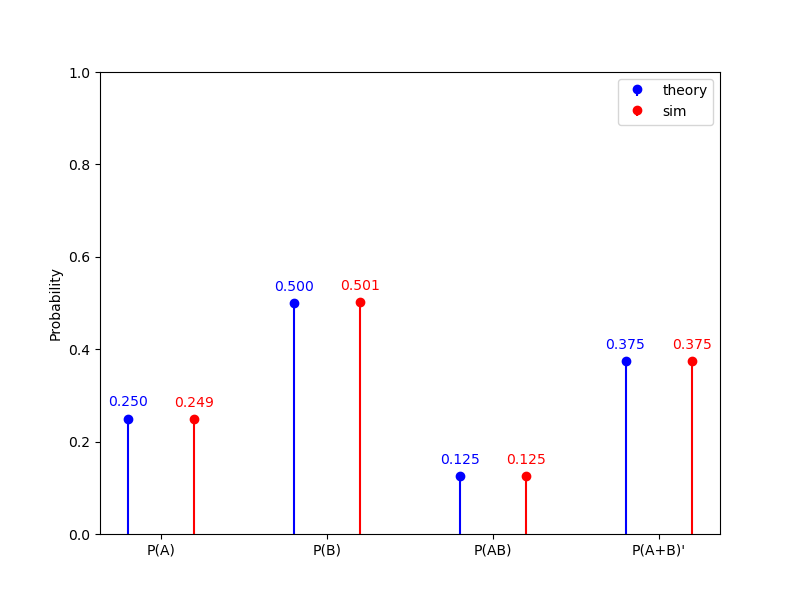
\includegraphics[width=0.7\textwidth]{figs/plot.png}
        \caption{Graphical representation of probabilities}
    \end{figure}
\end{frame}

\end{document}

